\documentclass[border=10pt]{standalone}
\usepackage{tikz}
\usetikzlibrary{shapes.geometric, arrows.meta, positioning, fit, backgrounds, shadows}

\definecolor{panelbg}{HTML}{ffffff}
\definecolor{accent1}{HTML}{c62828}
\definecolor{nodeblue}{HTML}{1565C0}
\definecolor{nodeorange}{HTML}{E65100}
\definecolor{nodegreen}{HTML}{2E7D32}
\definecolor{nodepurple}{HTML}{6A1B9A}
\definecolor{nodeteal}{HTML}{00695C}
\definecolor{textdark}{HTML}{1a1a2e}
\definecolor{textdim}{HTML}{455A64}
\definecolor{arrowgray}{HTML}{455A64}

\begin{document}
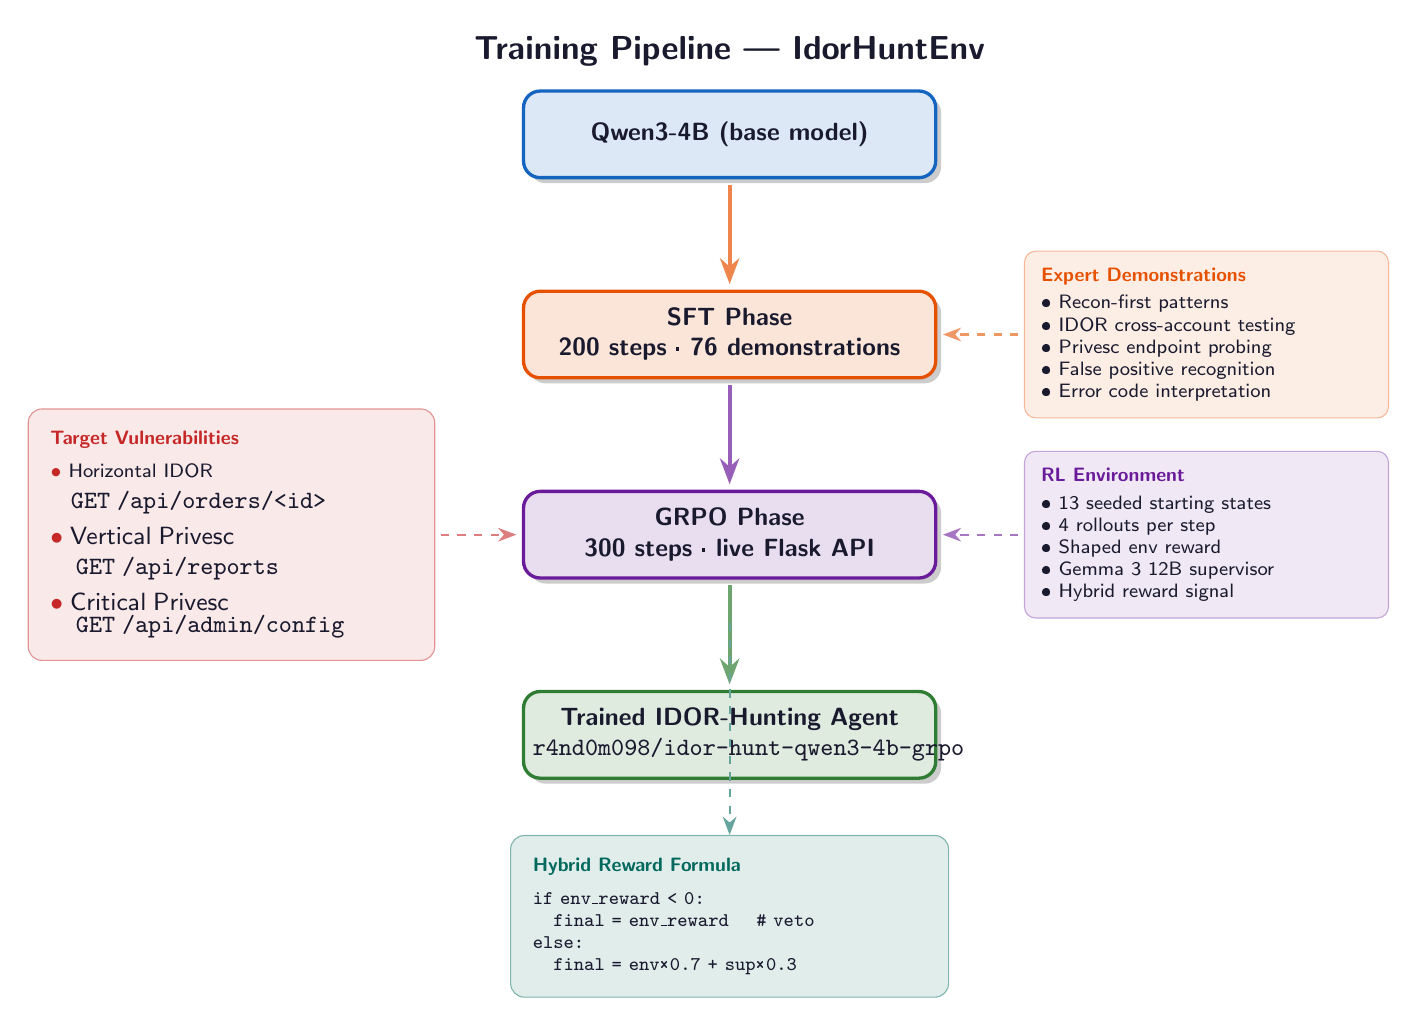
\begin{tikzpicture}[
  font=\sffamily,
  >=Stealth,
  node distance=0.7cm,
  every node/.style={text=textdark},
  phase/.style={
    rectangle, rounded corners=6pt,
    minimum width=5.2cm, minimum height=1.1cm,
    text width=5cm, align=center,
    draw, line width=1.2pt,
    font=\sffamily\bfseries\small,
    drop shadow={shadow xshift=2pt, shadow yshift=-2pt, opacity=0.4}
  },
  sidelabel/.style={
    rectangle, rounded corners=4pt,
    minimum width=4.4cm,
    text width=4.2cm, align=left,
    font=\sffamily\scriptsize,
    inner sep=6pt
  },
  arrowlabel/.style={
    font=\sffamily\tiny, text=textdim
  },
  connector/.style={
    ->, line width=1.4pt, color=arrowgray,
    shorten >=2pt, shorten <=2pt
  }
]

% ── Title ─────────────────────────────────────────────────────────────────
\node[text=textdark, font=\sffamily\bfseries\large] at (4.9, 0.55)
  {Training Pipeline — IdorHuntEnv};

% ── Phase nodes ───────────────────────────────────────────────────────────
\node[phase,
      fill=nodeblue!15!white, draw=nodeblue, text=textdark]
  (base) at (4.9, -0.5) {Qwen3-4B (base model)};

\node[phase,
      fill=nodeorange!15!white, draw=nodeorange, text=textdark,
      below=1.4cm of base]
  (sft) {SFT Phase\\\small 200 steps · 76 demonstrations};

\node[phase,
      fill=nodepurple!15!white, draw=nodepurple, text=textdark,
      below=1.4cm of sft]
  (grpo) {GRPO Phase\\\small 300 steps · live Flask API};

\node[phase,
      fill=nodegreen!15!white, draw=nodegreen, text=textdark,
      below=1.4cm of grpo]
  (final) {Trained IDOR-Hunting Agent\\
           \small\texttt{r4nd0m098/idor-hunt-qwen3-4b-grpo}};

% ── Arrows between phases ─────────────────────────────────────────────────
\draw[connector, color=nodeorange!70]  (base.south)  -- (sft.north);
\draw[connector, color=nodepurple!70] (sft.south)   -- (grpo.north);
\draw[connector, color=nodegreen!70]  (grpo.south)  -- (final.north);

% ── Side annotations — SFT ────────────────────────────────────────────────
\node[sidelabel,
      fill=nodeorange!10!white, draw=nodeorange!40, text=textdark,
      right=1.1cm of sft, yshift=0cm]
  (sft_ann) {%
    \textcolor{nodeorange}{\textbf{Expert Demonstrations}}\\[2pt]
    • Recon-first patterns\\
    • IDOR cross-account testing\\
    • Privesc endpoint probing\\
    • False positive recognition\\
    • Error code interpretation
  };

\draw[->, line width=0.8pt, color=nodeorange!60, dashed,
      shorten >=2pt, shorten <=2pt]
  (sft_ann.west) -- (sft.east);

% ── Side annotations — GRPO ───────────────────────────────────────────────
\node[sidelabel,
      fill=nodepurple!10!white, draw=nodepurple!40, text=textdark,
      right=1.1cm of grpo, yshift=0cm]
  (grpo_ann) {%
    \textcolor{nodepurple}{\textbf{RL Environment}}\\[2pt]
    • 13 seeded starting states\\
    • 4 rollouts per step\\
    • Shaped env reward\\
    • Gemma 3 12B supervisor\\
    • Hybrid reward signal
  };

\draw[->, line width=0.8pt, color=nodepurple!60, dashed,
      shorten >=2pt, shorten <=2pt]
  (grpo_ann.west) -- (grpo.east);

% ── Reward formula box ────────────────────────────────────────────────────
\node[rectangle, rounded corners=5pt,
      fill=nodeteal!12!white, draw=nodeteal!50,
      text=textdark, font=\sffamily\scriptsize,
      text width=5.0cm, align=left,
      inner sep=8pt,
      below=0.7cm of final]
  (reward) {%
    \textcolor{nodeteal}{\textbf{Hybrid Reward Formula}}\\[4pt]
    \texttt{if env\_reward < 0:}\\
    \quad\texttt{final = env\_reward \quad\# veto}\\
    \texttt{else:}\\
    \quad\texttt{final = env×0.7 + sup×0.3}
  };

\draw[->, line width=0.8pt, color=nodeteal!60, dashed]
  (grpo.south) ++(0,-0.55) -| (reward.north);

% ── Vulnerability targets ─────────────────────────────────────────────────
\node[rectangle, rounded corners=5pt,
      fill=accent1!10!white, draw=accent1!50,
      text=textdark, font=\sffamily\scriptsize,
      text width=4.6cm, align=left,
      inner sep=8pt,
      left=1.1cm of grpo, yshift=0cm]
  (vulns) {%
    \textcolor{accent1}{\textbf{Target Vulnerabilities}}\\[4pt]
    \textcolor{accent1}{$\bullet$} Horizontal IDOR\\
    \quad\small\texttt{GET /api/orders/<id>}\\[2pt]
    \textcolor{accent1}{$\bullet$} Vertical Privesc\\
    \quad\small\texttt{GET /api/reports}\\[2pt]
    \textcolor{accent1}{$\bullet$} Critical Privesc\\
    \quad\small\texttt{GET /api/admin/config}
  };

\draw[->, line width=0.8pt, color=accent1!60, dashed,
      shorten >=2pt, shorten <=2pt]
  (vulns.east) -- (grpo.west);

\end{tikzpicture}
\end{document}
